\section*{Materiale}

Il materiale utilizzato per questa esperienza di laboratorio è il sguente:

\begin{itemize} \itemsep0pt \parskip0pt \parsep0pt
    \item{Breadboard, cavetti, cavi a banana per le connessioni, cavi con calza e 3 elettrodi per la misura;}
    \item{Amplificatore operazionale OP07 a 8 pin e Amplificatore di isolamento ISO124;}
    \item{Amplificatore per strumentazione AD622 a 8 pin;}
    \item{Capacità da \SI{10}{\nano\farad}, \SI{47}{\nano\farad}, \SI{100}{\nano\farad} e Resistenze varie: \SI{220}{\ohm}, \SI{3.9}{\kilo\ohm}, \SI{10}{\kilo\ohm}, \SI{100}{\kilo\ohm};}
    \item{Alimentatore di tensione continua e 2 batterie da \SI{9}{\volt};}
    \item{Generatore di funzioni d'onda: Agilent 33120A e Multimetro: Agilent Technologies 34410A;}
    \item{Oscilloscopio: Agilent DSO-X 2002A;}
\end{itemize}

Facciamo presente che sui valori di resistenza riportati in tutto l'elaborato non abbiamo riportato la loro incertezza per motivi di chiarezza e leggibilità dello scritto. Tuttavia abbiamo assunto un errore del $5\%$ sul valore nominale delle resistenze.

\section*{Circuito}

\begin{figure}[H]
    \centering
	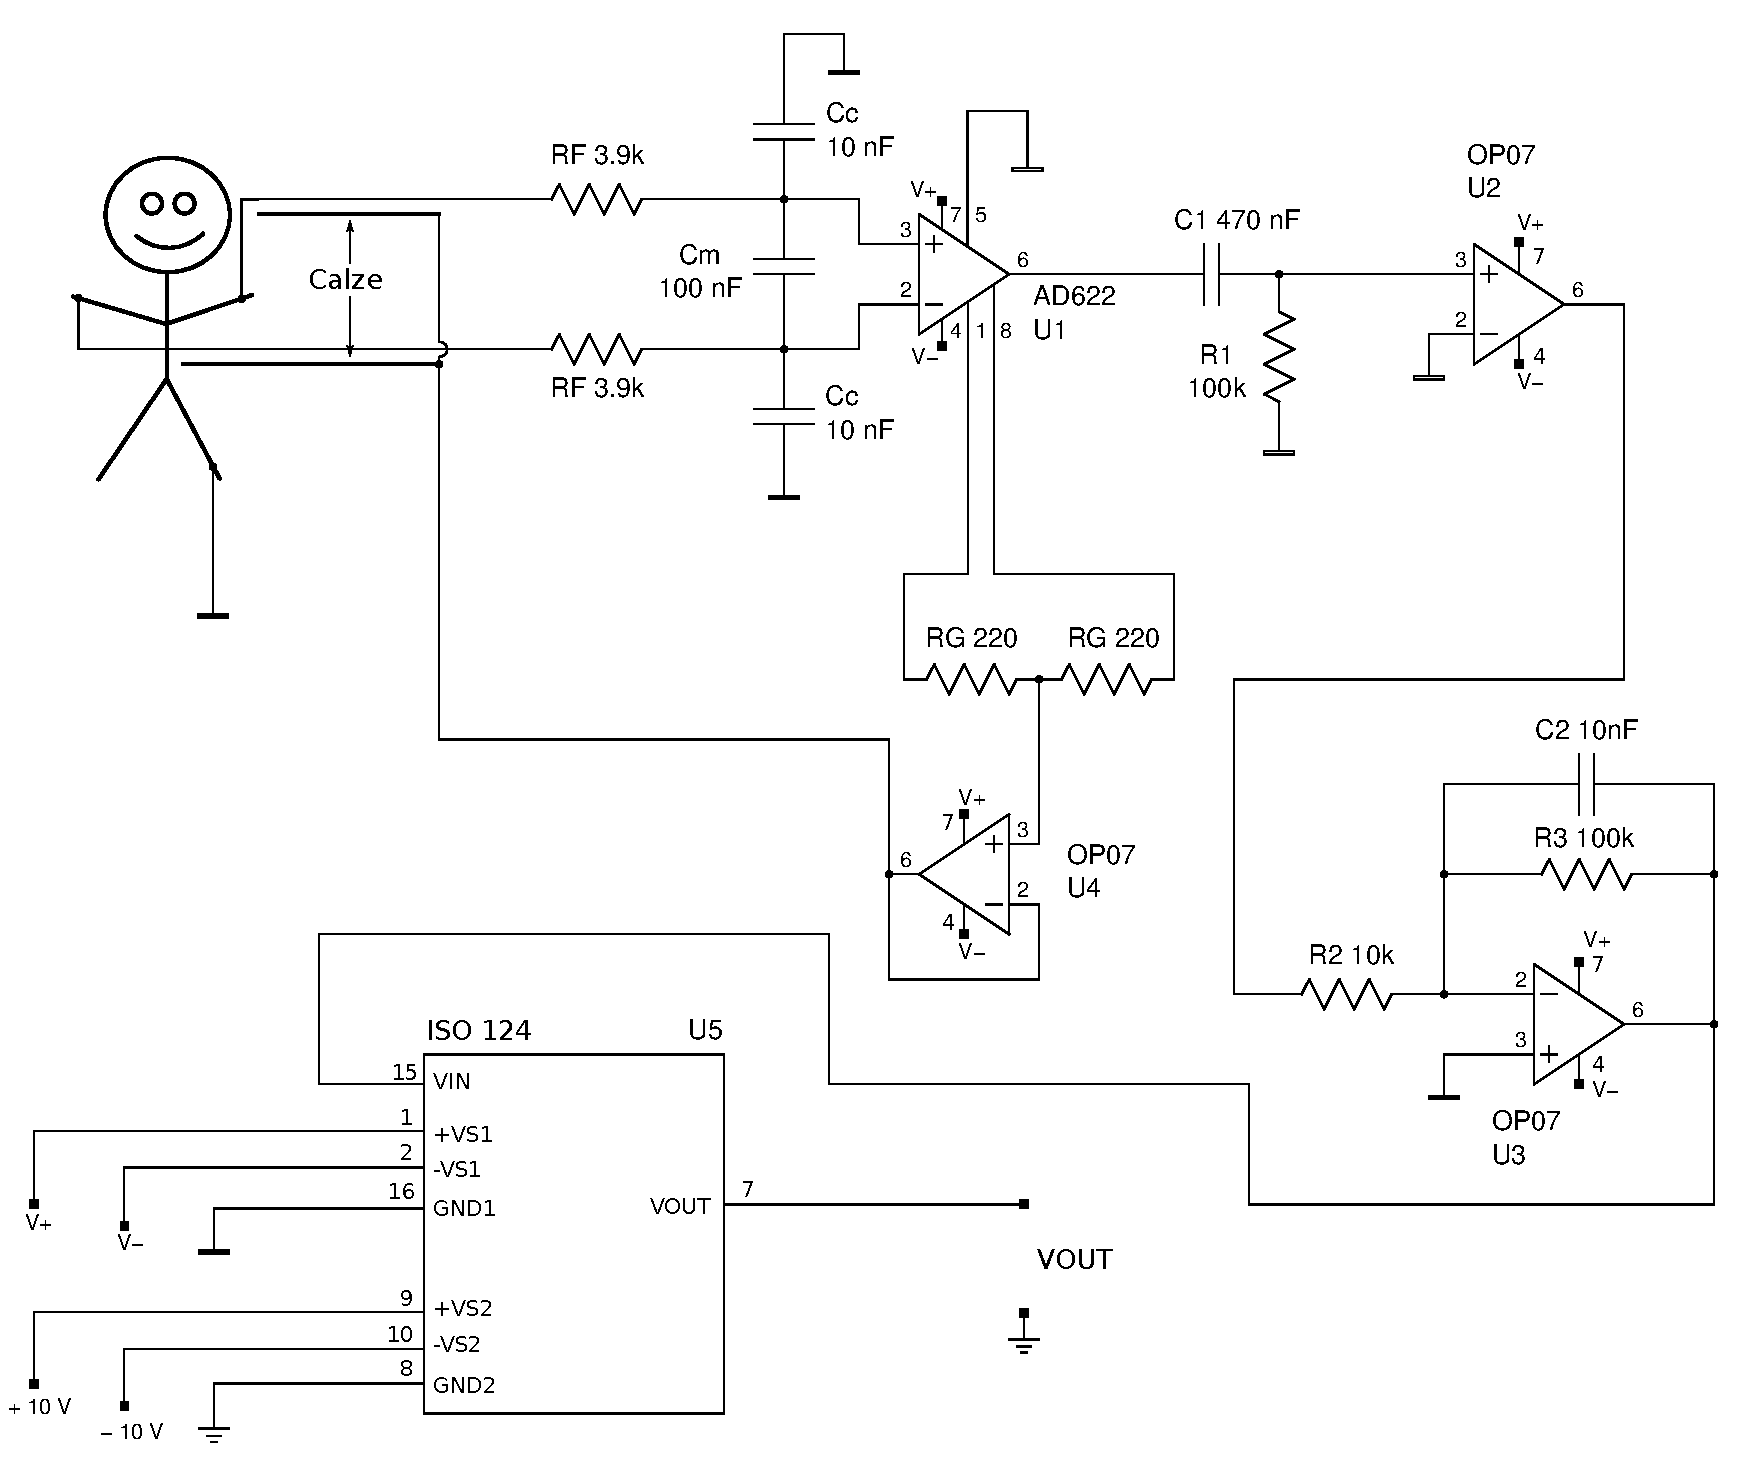
\includegraphics[width=0.87\textwidth]{figure/s.pdf}
	\caption{Circuito per la misura dell'ECG}
	\label{fig:ecg}
\end{figure}

%\begin{figure}[h]
%        \centering
%        \begin{subfigure}[b]{0.45\textwidth}
%        	\def\svgwidth{\textwidth}
%                \subimport{Figure/}{slew_circ.pdf_tex}
%                \caption{Circuito usato per misurare lo Slew Rate dell'amplificatore operazionale. E' un circuito in configurazione emitter follower, con circuito di retroazione negativo.}
%                \label{fig:slew_rate}
%        \end{subfigure}
%        ~
%        \begin{subfigure}[b]{0.45\textwidth}
%        	\def\svgwidth{\textwidth}
%                \subimport{Figure/}{max_curr_circ.pdf_tex}
%                \caption{Circuito usato per misurare il valore della corrente massima generabile dall'amplificatore. L'amplificatore operazionale è usato in configurazione emitter follower con circuito di retroazione negativo.}
%                \label{fig:current}
%        \end{subfigure}
%        \caption{}
%\end{figure}
